\documentclass[aspectratio=169, handout]{beamer}

%\usepackage[table]{xcolor}
\mode<presentation> {
\setbeamercovered{transparent}
  \usetheme{Boadilla}

\renewcommand{\familydefault}{cmss}
\usepackage{bm}
\usepackage{listings}
\useinnertheme{rectangles}
}
\usepackage{amsmath}
\usepackage{bbold}
\usepackage{tcolorbox}
\setbeamercolor{normal text}{fg=black}
\setbeamercolor{structure}{fg= blue}
\definecolor{trial}{cmyk}{1,0,0, 0}
\definecolor{trial2}{cmyk}{0.00,0,1, 0}
\definecolor{darkgreen}{rgb}{0,.4, 0.1}
\definecolor{darkpurple}{rgb}{0.4, 0, 0.6}
\usepackage{array}
\beamertemplatesolidbackgroundcolor{white}  \setbeamercolor{alerted
text}{fg=darkpurple}
\setbeamertemplate{caption}[numbered]\newcounter{mylastframe}

\font\domino=domino
\def\die#1{{\domino#1}}
\usepackage{tikz}
\usetikzlibrary{arrows}
\usepackage{colortbl}

\renewcommand{\familydefault}{cmss}

\usepackage{tikz}
\usepackage{lipsum}
\usepackage{booktabs}

\lstset{%
  language=R,
  basicstyle=\ttfamily\small,
  keywordstyle=\color{blue},
  commentstyle=\color{darkgreen},
  stringstyle=\color{darkpurple},
  showstringspaces=false,
  breaklines=true,
  frame=single,
  backgroundcolor=\color{gray!10}
}

 \newenvironment{changemargin}[3]{%
 \begin{list}{}{%
 \setlength{\topsep}{0pt}%
 \setlength{\leftmargin}{#1}%
 \setlength{\rightmargin}{#2}%
 \setlength{\topmargin}{#3}%
 \setlength{\listparindent}{\parindent}%
 \setlength{\itemindent}{\parindent}%
 \setlength{\parsep}{\parskip}%
 }%
\item[]}{\end{list}}
\usetikzlibrary{arrows}
\usetikzlibrary{arrows.meta, positioning}
\usepackage{pgfplots}
\pgfplotsset{compat=1.17}
\usecolortheme{lily}

\newtheorem{com}{Comment}
\newtheorem{lem} {Lemma}
\newtheorem{prop}{Proposition}
\newtheorem{condition}{Condition}
\newtheorem{thm}{Theorem}
\newtheorem{defn}{Definition}
\newtheorem{cor}{Corollary}
\newtheorem{obs}{Observation}
 \numberwithin{equation}{section}

\makeatletter
\def\beamerorig@set@color{%
  \pdfliteral{\current@color}%
  \aftergroup\reset@color
}
\def\beamerorig@reset@color{\pdfliteral{\current@color}}
\makeatother
\setbeamertemplate{navigation symbols}{}

\useoutertheme{miniframes}
\title[PLSC 30700]{Linear Models Lecture 15: GMM Estimation and Efficiency}

\author{Robert Gulotty}
\institute[Chicago]{University of Chicago}
\vspace{0.3in}


\begin{document}

%========================================================
% SECTION 1: MOTIVATION
%========================================================
\section{Motivation}

%--- Slide 1: Title ---
\begin{frame}
\titlepage
\end{frame}

%--- Slide 2: Where We Left Off ---
\begin{frame}{Where We Left Off}

In Lecture 14, we introduced IV estimation as a \alert{method of moments}:
$$\frac{1}{n}\sum_{i=1}^n Z_i(Y_i - X_i'\beta) = 0$$

\medskip
This works when the number of moment conditions $\ell$ equals the number of parameters $k$.

\medskip
\alert{But what if we have more instruments than parameters?}

\begin{itemize}
\item We cannot simultaneously set all moment conditions to zero
\item We need a principled way to \textit{get as close as possible}
\item This is the \textbf{overidentification problem}
\end{itemize}

\end{frame}

%--- Slide 3: Three Reasons to Learn GMM ---
\begin{frame}{Three Reasons to Learn GMM}

\begin{tcolorbox}[colback=blue!5, colframe=blue!50, title=\textbf{Three Meta-Lessons from GMM}]
\begin{enumerate}
\item \textbf{Semiparametric:} GMM requires only moment conditions --- no distributional assumptions. It achieves the \textit{semiparametric efficiency bound} (Chamberlain, 1987).

\medskip
\item \textbf{Efficient:} The optimal weight matrix minimizes asymptotic variance across all GMM estimators. Two-step and iterated GMM achieve this bound in practice.

\medskip
\item \textbf{General:} GMM provides a unified framework for estimation \textit{and} testing. It nests OLS, GLS, IV, and 2SLS as special cases --- and extends to nonlinear models and treatment effect heterogeneity.
\end{enumerate}
\end{tcolorbox}

\end{frame}

%--- Slide 4: Moment Equation Models (Hansen 13.2) ---
\begin{frame}{Moment Equation Models (Hansen \S13.2)}

Let $g_i(\beta)$ be a known $\ell \times 1$ function of the $i^{th}$ observation and a $k \times 1$ parameter $\beta$.

\begin{defn}
A \textbf{moment equation model} is defined by
$$\mathbb{E}[g_i(\beta)] = 0$$
and a parameter space $\beta \in B$.
\end{defn}

\medskip
\textbf{Identification requires $\ell \geq k$:}
\begin{itemize}
\item $\ell = k$: \textbf{Just identified} --- exactly enough information
\item $\ell > k$: \textbf{Overidentified} --- excess information (testable restrictions)
\item $\ell < k$: \textbf{Underidentified} --- insufficient information
\end{itemize}

\smallskip
\textbf{Example:} IV model: $g_i(\beta) = Z_i(Y_i - X_i'\beta)$

\end{frame}

%--- Slide 5: Everything Is a Moment Condition ---
\begin{frame}{Everything Is a Moment Condition}

\begin{table}[h]
\centering
\small
\begin{tabular}{lll}
\toprule
\textbf{Estimator} & \textbf{Moment condition $g_i(\beta)$} & \textbf{MME} \\
\midrule
Sample mean & $Y_i - \mu$ & $\hat\mu = \bar{Y}$ \\[4pt]
OLS & $X_i(Y_i - X_i'\beta)$ & $\hat\beta = (X'X)^{-1}X'Y$ \\[4pt]
IV & $Z_i(Y_i - X_i'\beta)$ & $\hat\beta = (Z'X)^{-1}Z'Y$ \\[4pt]
2SLS & $Z_i(Y_i - X_i'\beta)$ with $W=(Z'Z)^{-1}$ & $\hat\beta_{2SLS}$ \\[4pt]
GLS & $\bar X_i\Sigma^{-1}(Y_i - \bar X_i'\beta)$ & $\hat\beta_{GLS}$ \\
\bottomrule
\end{tabular}
\end{table}

\medskip
\begin{tcolorbox}[colback=blue!5, colframe=blue!50]
\textbf{Key insight:} All the estimators we have studied are \textit{method of moments estimators} --- they solve $\bar{g}_n(\hat\beta) = 0$. GMM generalizes to the overidentified case.
\end{tcolorbox}

\end{frame}

%========================================================
% SECTION 2: THE GMM ESTIMATOR
%========================================================
\section{The GMM Estimator}

%--- Slide 6: The Overidentification Problem (Hansen 13.4) ---
\begin{frame}{The Overidentification Problem (Hansen \S13.4)}

Define the sample moment:
$$\bar{g}_n(\beta) = \frac{1}{n}\sum_{i=1}^n g_i(\beta)$$

\smallskip
When $\ell = k$: We can solve $\bar{g}_n(\hat\beta) = 0$ exactly.

\smallskip
When $\ell > k$: There are \alert{more equations than unknowns}. In general, no $\beta$ sets $\bar{g}_n(\beta) = 0$.

\medskip
\textbf{Intuition:} Think of $\mu = Z'Y$, $G = Z'X$, and $\eta = \mu - G\beta$. We want $\eta$ small. Regressing $\mu$ on $G$:
$$\tilde\beta = (G'G)^{-1}G'\mu$$
minimizes $\eta'\eta$. But we can do \textit{better} with weighted least squares...

\end{frame}

%--- Slide 7: The GMM Criterion Function ---
\begin{frame}{The GMM Criterion Function}

For a positive definite $\ell \times \ell$ weight matrix $W$, the \textbf{GMM criterion function} is:

$$\boxed{J(\beta) = n\,\bar{g}_n(\beta)' W\, \bar{g}_n(\beta)}$$

\medskip
\begin{itemize}
\item $J(\beta) \geq 0$ for all $\beta$ (since $W > 0$)
\item When $W = I_\ell$: $J(\beta) = n\|\bar{g}_n(\beta)\|^2$ (Euclidean distance)
\item The factor $n$ is for distributional convenience
\item \alert{Different choices of $W$ yield different estimators} --- and different efficiency
\end{itemize}

\smallskip
For the linear IV model:
$$J(\beta) = n(Z'Y - Z'X\beta)' W (Z'Y - Z'X\beta)$$

\end{frame}

%--- Slide 8: The GMM Estimator (Hansen Def 13.1, Thm 13.1) ---
\begin{frame}{The GMM Estimator (Hansen Def.~13.1, Thm.~13.1)}

\begin{defn}[GMM Estimator]
$$\hat\beta_{\text{gmm}} = \arg\min_\beta J(\beta) = \arg\min_\beta\; n\,\bar{g}_n(\beta)' W\, \bar{g}_n(\beta)$$
\end{defn}

\bigskip
\begin{thm}[13.1]
For the overidentified linear IV model, the GMM estimator is:
$$\hat\beta_{\text{gmm}} = (X'ZWZ'X)^{-1}(X'ZWZ'Y)$$
\end{thm}

\bigskip
\begin{itemize}
\item When $\ell = k$ (just identified): $\hat\beta_{\text{gmm}} = (Z'X)^{-1}(Z'Y) = \hat\beta_{\text{iv}}$, regardless of $W$
\item When $\ell > k$: the estimator \alert{depends on $W$}
\end{itemize}

\end{frame}

%--- Slide 9: 2SLS as GMM (Thm 13.2) ---
\begin{frame}{2SLS as GMM (Hansen Thm.~13.2)}

\begin{thm}[13.2]
If $W = (Z'Z)^{-1}$, then $\hat\beta_{\text{gmm}} = \hat\beta_{\text{2sls}}$.

Furthermore, if $k = \ell$ then $\hat\beta_{\text{gmm}} = \hat\beta_{\text{iv}}$.
\end{thm}

\medskip
\textbf{Proof sketch:} Substitute $W = (Z'Z)^{-1}$ into Theorem 13.1:
\begin{align*}
\hat\beta &= (X'Z(Z'Z)^{-1}Z'X)^{-1}(X'Z(Z'Z)^{-1}Z'Y) = (X'P_ZX)^{-1}(X'P_ZY)
\end{align*}
where $P_Z = Z(Z'Z)^{-1}Z'$ is the projection matrix --- exactly the 2SLS formula.

\medskip
\begin{tcolorbox}[colback=blue!5, colframe=blue!50]
\textbf{Takeaway:} 2SLS is a \textit{one-step} GMM estimator. But $(Z'Z)^{-1}$ is not always the best weight matrix.
\end{tcolorbox}

\end{frame}

%--- Slide 10: Asymptotic Distribution (Thm 13.3) ---
\begin{frame}{Asymptotic Distribution (Hansen Thm.~13.3)}

Let $Q = \mathbb{E}[ZX']$ and $\Omega = \mathbb{E}[ZZ'e^2]$.

\begin{thm}[13.3: Asymptotic Distribution of GMM]
As $n \to \infty$,
$$\sqrt{n}(\hat\beta_{\text{gmm}} - \beta) \xrightarrow{d} N(0, V_\beta)$$
where
$$\boxed{V_\beta = (Q'WQ)^{-1}(Q'W\Omega WQ)(Q'WQ)^{-1}}$$
\end{thm}

\bigskip
\begin{itemize}
\item This is a \textbf{sandwich form}: ``bread'' $(Q'WQ)^{-1}$ wraps ``meat'' $Q'W\Omega WQ$
\item Applies for \textit{any} positive definite weight matrix $W$
\item Different $W$ $\Rightarrow$ different $V_\beta$ $\Rightarrow$ different efficiency
\end{itemize}

\end{frame}

%--- Slide 11: What Is the Best Weighting? ---
\begin{frame}{What Is the Best Weighting?}

\textbf{Question:} Which $W$ minimizes $V_\beta$?

\bigskip
\textbf{Intuition:} We want to weight moments that are
\begin{itemize}
\item \textit{more informative} (high signal) $\Rightarrow$ weight up
\item \textit{less noisy} (low variance) $\Rightarrow$ weight up
\end{itemize}

\bigskip
The variance of the sample moments is $\Omega = \mathbb{E}[g_ig_i']$. So \alert{weight inversely to their variance}: $W = \Omega^{-1}$.

\bigskip
\textbf{Analogy:} Just like GLS weights observations by the inverse of $\text{Var}(e_i)$, efficient GMM weights \textit{moment conditions} by the inverse of their covariance.

\end{frame}

%--- Slide 12: Efficient GMM (Thms 13.4--13.5) ---
\begin{frame}{Efficient GMM (Hansen Thms.~13.4--13.5)}

\begin{thm}[13.4: Efficient GMM]
Setting $W = \Omega^{-1}$, as $n\to\infty$:
$\sqrt{n}(\hat\beta_{\text{gmm}} - \beta) \xrightarrow{d} N(0, V_\beta)$ where $V_\beta = (Q'\Omega^{-1}Q)^{-1}$.
\end{thm}

The sandwich \alert{collapses}: $(Q'\Omega^{-1}Q)^{-1}(\underbrace{Q'\Omega^{-1}\Omega \Omega^{-1}Q}_{Q'\Omega^{-1}Q})(Q'\Omega^{-1}Q)^{-1}$

\smallskip
\begin{thm}[13.5: Efficiency]
For any $W > 0$:
$(Q'WQ)^{-1}(Q'W\Omega WQ)(Q'WQ)^{-1} - (Q'\Omega^{-1}Q)^{-1} \geq 0$.
\end{thm}

\smallskip
\begin{tcolorbox}[colback=blue!5, colframe=blue!50]
No GMM estimator with these moment conditions can have a smaller asymptotic variance. Chamberlain (1987): this is the \textbf{semiparametric efficiency bound}.
\end{tcolorbox}

\end{frame}

%========================================================
% SECTION 3: 2SLS vs. EFFICIENT GMM
%========================================================
\section{2SLS vs.\ Efficient GMM}

%--- Slide 13: When Is 2SLS Efficient? (Thm 13.6) ---
\begin{frame}{When Is 2SLS Efficient? (Hansen Thm.~13.6)}

Recall 2SLS uses $W = (Z'Z)^{-1}$, which converges to $(\mathbb{E}[ZZ'])^{-1}$.

\medskip
The efficient weight is $\Omega^{-1} = (\mathbb{E}[ZZ'e^2])^{-1}$.

\medskip
These are equal when $\mathbb{E}[e^2 | Z] = \sigma^2$ (conditional homoskedasticity):
$$\mathbb{E}[ZZ'e^2] = \sigma^2 \mathbb{E}[ZZ']$$

\begin{thm}[13.6]
Under conditional homoskedasticity $\mathbb{E}[e^2 | Z] = \sigma^2$, the 2SLS estimator $\hat\beta_{\text{2sls}}$ is efficient GMM.
\end{thm}

\smallskip
\alert{Implications:}
\begin{itemize}
\item Homoskedastic errors $\Rightarrow$ 2SLS is fine, no need for GMM
\item Heteroskedastic errors $\Rightarrow$ 2SLS is \textit{inefficient}; use efficient GMM
\end{itemize}

\end{frame}

%--- Slide 14: Two-Step GMM (Hansen 13.10, Thm 13.7) ---
\begin{frame}{Two-Step GMM (Hansen \S13.10, Thm.~13.7)}

\textbf{Problem:} $\Omega = \mathbb{E}[ZZ'e^2]$ is unknown. We need to estimate it.

\medskip
\textbf{Two-Step GMM:}
\begin{enumerate}
\item \textbf{Step 1:} Estimate $\beta$ by 2SLS (using $W = (Z'Z)^{-1}$). Compute residuals $\tilde{e}_i = Y_i - X_i'\hat\beta_{\text{2sls}}$.
\item \textbf{Step 2:} Estimate $\hat\Omega = \frac{1}{n}\sum_{i=1}^n Z_iZ_i'\tilde{e}_i^2$, set $\hat{W} = \hat\Omega^{-1}$, and re-estimate $\beta$.
\end{enumerate}

\begin{thm}[13.7]
The two-step GMM estimator is asymptotically efficient:
$$\sqrt{n}(\hat\beta_{\text{gmm}} - \beta) \xrightarrow{d} N(0, V_\beta)\quad\text{where}\quad V_\beta = (Q'\Omega^{-1}Q)^{-1}$$
\end{thm}

\textbf{Key point:} The initial estimator does not affect the asymptotic distribution.

\end{frame}

%--- Slide 15: Iterated GMM (Hansen 13.11) ---
\begin{frame}{Iterated GMM (Hansen \S13.11)}

The two-step estimator's \textit{finite-sample} performance can depend on the initial estimator. To remove this dependence:

\medskip
\textbf{Iterated GMM:}
\begin{enumerate}
\item Start with $\hat\beta^{(0)}$ (e.g., 2SLS)
\item Compute $\hat\Omega^{(s)} = \frac{1}{n}\sum Z_iZ_i'(\hat e_i^{(s)})^2$
\item Re-estimate: $\hat\beta^{(s+1)} = (X'Z\hat\Omega^{(s)-1}Z'X)^{-1}(X'Z\hat\Omega^{(s)-1}Z'Y)$
\item Repeat until convergence
\end{enumerate}

\medskip
In R's \texttt{gmm} package: \texttt{type = "twoStep"} (two-step) or \texttt{type = "iterative"} (iterated).

\medskip
\textbf{Note:} Hansen and Lee (2021) show the iterated GMM estimator is unaffected by whether the weight matrix is computed with or without centering.

\end{frame}

%--- Slide 16: Covariance Matrix Estimation (Hansen 13.12) ---
\begin{frame}{Covariance Matrix Estimation (Hansen \S13.12)}

\textbf{One-step or two-step GMM} (general $W$):
$$\hat V_\beta = (\hat Q'\hat W\hat Q)^{-1}(\hat Q'\hat W\hat\Omega\hat W\hat Q)(\hat Q'\hat W\hat Q)^{-1}$$
where $\hat Q = \frac{1}{n}\sum Z_iX_i'$ and $\hat\Omega$ uses residuals from the final step.

\medskip
\textbf{Efficient iterated GMM} ($\hat W = \hat\Omega^{-1}$):
$$\hat V_\beta = \left(\hat Q'\hat\Omega^{-1}\hat Q\right)^{-1}$$
The sandwich simplifies --- just like GLS vs.\ OLS variance formulas.

\medskip
\begin{tcolorbox}[colback=blue!5, colframe=blue!50]
\textbf{Practical advice:} Always report robust (sandwich) standard errors for one-step GMM. For efficient GMM, the simplified formula is already robust.
\end{tcolorbox}

\end{frame}

%========================================================
% SECTION 4: MISSING DATA APPLICATION
%========================================================
\section{Application: Missing Data}

%--- Slide 17: Why Missing Data Needs GMM ---
\begin{frame}{Why Missing Data Needs GMM}

\textbf{Meta-lesson \#1: GMM is semiparametric.}

\medskip
Missing data on regressors is pervasive (Abrevaya \& Donald 2017, surveying top journals 2006--2008): $\sim$50\% of empirical papers in JLE/QJE have missing data; $\sim$70\% use the \textit{complete case method} (drop observations).

\medskip
\textbf{Standard approaches:}
\begin{enumerate}
\item \textbf{Complete case:} Drop missing obs. --- loses efficiency
\item \textbf{Dummy variable:} Fill in 0, add indicator --- \alert{can be inconsistent}
\item \textbf{Linear imputation:} Predict missing values --- requires extra assumptions
\end{enumerate}

\medskip
\alert{GMM offers a better way:} Exploit moment conditions from \textit{both} complete and incomplete observations simultaneously.

\end{frame}

%--- Slide 18: The Missing Data Model (Abrevaya 2017) ---
\begin{frame}{The Missing Data Model (Abrevaya \& Donald, 2017)}

\textbf{Structural regression:}
$$y_i = \alpha_0 x_i + z_i'\beta_0 + \varepsilon_i \qquad \text{where } E(x_i\varepsilon_i) = 0,\; E(z_i\varepsilon_i) = 0$$

$x_i$ is a (possibly missing) scalar regressor; $z_i$ is always observed.

\medskip
\textbf{Linear projection of $x_i$ on $z_i$:}
$x_i = z_i'\gamma_0 + \xi_i$ where $E(z_i\xi_i) = 0$.
\textbf{Missingness indicator:} $m_i = 1$ if $x_i$ missing, $m_i = 0$ if observed.

\medskip
\textbf{Key substitution:} For observations with $m_i = 1$:
$$y_i = z_i'(\gamma_0\alpha_0 + \beta_0) + (\varepsilon_i + \xi_i\alpha_0) \equiv z_i'\delta_0 + \eta_i$$

\medskip
\textbf{Assumption 1:} (a) $E(m_iz_i\varepsilon_i) = 0$; (b) $E(m_iz_i\xi_i) = 0$; (c) $E(m_ix_i\varepsilon_i) = 0$.

$\Rightarrow$ Missingness may depend on $z_i$ but not on $\varepsilon_i$ or $\xi_i$.
\end{frame}

%--- Slide 19: Three Blocks of Moment Conditions ---
\begin{frame}{Three Blocks of Moment Conditions}

The parameters are $\theta = (\alpha_0, \beta_0, \gamma_0)'$ with $k = 2K+1$ unknowns.

\medskip
\textbf{Block 1} (observed cases, structural equation):
$(1-m_i)\cdot w_i(y_i - \alpha_0 x_i - z_i'\beta_0) = 0$ \hfill [$K+1$ conditions]

\textbf{Block 2} (observed cases, projection equation):
$(1-m_i)\cdot z_i(x_i - z_i'\gamma_0) = 0$ \hfill [$K$ conditions]

\textbf{Block 3} (missing cases, substituted equation):
$m_i \cdot z_i(y_i - z_i'(\gamma_0\alpha_0 + \beta_0)) = 0$ \hfill [$K$ conditions]

\medskip
\textbf{Total:} $\ell = 3K + 1$ moments for $k = 2K + 1$ parameters $\Rightarrow$ $K$ \alert{overidentifying restrictions} (testable via J-test!)

\smallskip
With $K = 2$ (intercept + IQ): 7 moments, 5 parameters, \textbf{2 overidentifying restrictions}

\end{frame}

%--- Slide 20: Why GMM Beats the Alternatives ---
\begin{frame}{Why GMM Beats the Alternatives}

\vspace{-4pt}
{\footnotesize
\begin{table}[h]
\centering
\begin{tabular}{lccc}
\toprule
\textbf{Method} & \textbf{Consistent?} & \textbf{Efficient?} & \textbf{Testable?} \\
\midrule
Complete case & Yes (drops $m_i\!=\!1$) & No (fewer obs) & No \\
Dummy variable & \alert{Sometimes no} & No & No \\
Linear imputation & Yes (under Assn 1) & Somewhat & No \\
\textbf{GMM} & \textbf{Yes} (under Assn 1) & \textbf{Yes} (optimal $W$) & \textbf{Yes} (J-test) \\
\bottomrule
\end{tabular}
\end{table}
}

\smallskip
\textbf{Abrevaya \& Donald Monte Carlo} ($n=400$, 1000 replications):

{\footnotesize
\begin{table}[h]
\centering
\begin{tabular}{lccc}
\toprule
\textbf{Method} & \textbf{Bias ($\alpha_0$)} & \textbf{$n \times$Var ($\alpha_0$)} & \textbf{MSE ($\alpha_0$)} \\
\midrule
Complete case & 0.011 & 13.93 & 0.035 \\
Dummy variable & $-0.194$ & 13.94 & 0.073 \\
FGLS & 0.011 & 13.93 & 0.035 \\
\textbf{GMM} & \textbf{0.006} & \textbf{12.53} & \textbf{0.031} \\
\bottomrule
\end{tabular}
\end{table}
}

\end{frame}

%--- Slide 21: WLS Data (R code) ---
\begin{frame}[fragile]{WLS Data: Education and BMI}

\begin{lstlisting}[basicstyle=\ttfamily\footnotesize]
library(gmm); library(haven); library(estimatr)

# Wisconsin Longitudinal Study data
data1 <- read_dta("wls-data.dta")
data_men <- subset(data1, male == 1)

# How much data is missing?
table(data_men$bmimissing)
#  0    1
# 4231 1095   (~21% missing)

# Complete-case regression
data_complete <- subset(data_men, bmimissing == 0)
cc_reg <- lm(educ ~ bmirating + iq, data = data_complete)
\end{lstlisting}

\smallskip
\textbf{Question:} Education ($y$) regressed on BMI rating ($x$, sometimes missing) and IQ ($z$, always observed).

\end{frame}

%--- Slide 22: Defining GMM Moment Functions in R ---
\begin{frame}[fragile]{Defining GMM Moment Functions in R}

\begin{lstlisting}[basicstyle=\ttfamily\scriptsize]
g_men <- function(theta, x) {
  beta_0 <- theta[1]; alpha <- theta[2]; beta_iq <- theta[3]
  gamma_0 <- theta[4]; gamma_iq <- theta[5]
  educ <- x[,1]; bmirating <- x[,2]; iq <- x[,3]; bmimissing <- x[,4]

  # Block 1: structural eq (observed cases)
  r1 <- (1 - bmimissing) * (educ - beta_0 - alpha*bmirating - beta_iq*iq)
  # Block 2: projection eq (observed cases)
  r2 <- (1 - bmimissing) * (bmirating - gamma_0 - gamma_iq*iq)
  # Block 3: substituted eq (missing cases)
  r3 <- bmimissing * (educ - (gamma_0*alpha+beta_0) - (gamma_iq*alpha+beta_iq)*iq)

  cbind(r1, r1*bmirating, r1*iq,  # 3 moments
        r2, r2*iq,                  # 2 moments
        r3, r3*iq)                  # 2 moments = 7 total, 5 params
}
\end{lstlisting}

\end{frame}

%--- Slide 23: Running GMM in R ---
\begin{frame}[fragile]{Running GMM in R}

\begin{lstlisting}[basicstyle=\ttfamily\footnotesize]
# Starting values from complete-case regressions
start_men <- c(beta_0 = coef(cc_reg)[1],
               alpha  = coef(cc_reg)[2],
               beta_iq = coef(cc_reg)[3],
               gamma_0 = coef(proj_reg)[1],
               gamma_iq = coef(proj_reg)[2])

# Two-step GMM with HAC variance
gmm_men <- gmm(g_men, x = x_men, t0 = start_men,
                type = "twoStep",
                wmatrix = "ident", vcov = "HAC")
summary(gmm_men)
\end{lstlisting}

\smallskip
\textbf{Key arguments:}
\begin{itemize}\itemsep=1pt
\item \texttt{type = "twoStep"}: Initial $W = I$, then update with $\hat\Omega^{-1}$
\item \texttt{wmatrix = "ident"}: First-step weight matrix is identity
\item \texttt{vcov = "HAC"}: HAC variance estimator
\end{itemize}

\end{frame}

%--- Slide 24: Comparing Methods: Results ---
\begin{frame}[fragile]{Comparing Methods: Results}

\begin{table}[h]
\centering
\begin{tabular}{lccc}
\toprule
& \textbf{Complete Case} & \textbf{Dummy Variable} & \textbf{GMM} \\
\midrule
$\hat\alpha$ (BMI) & $-0.0343$ & $-0.0343$ & $-0.0340$ \\
SE & $(0.0077)$ & $(0.0073)$ & $(0.0072)$ \\[4pt]
$\hat\beta_{IQ}$ & $0.0563$ & $0.0567$ & $0.0564$ \\
SE & $(0.0017)$ & $(0.0015)$ & $(0.0015)$ \\[4pt]
$n$ used & 4231 & 5326 & 5326 \\
\bottomrule
\end{tabular}
\end{table}

\medskip
\textbf{J-test for overidentifying restrictions:}
\begin{lstlisting}[basicstyle=\ttfamily\footnotesize]
specTest(gmm_men)  # J-test = ?, df = 2, p-value = ?
\end{lstlisting}

\begin{itemize}
\item Large p-value: fail to reject $\Rightarrow$ Assumption 1 is plausible
\item Small p-value: evidence against the linear projection restriction
\end{itemize}

\end{frame}

%========================================================
% SECTION 5: NONLINEAR GMM AND SUMMARY
%========================================================
\section{Nonlinear GMM and Summary}

%--- Slide 25: Nonlinear GMM (Hansen 13.25) ---
\begin{frame}{Nonlinear GMM (Hansen \S13.25)}

So far: $g_i(\beta)$ is linear in $\beta$. In general, $g_i(\beta)$ can be \textbf{nonlinear}.

\medskip
The GMM estimator still minimizes $J(\beta) = n\,\bar{g}_n(\beta)'\hat W\,\bar{g}_n(\beta)$ but now requires numerical optimization (no closed form).

\medskip
\begin{block}{Proposition 13.1: Distribution of Nonlinear GMM}
$\sqrt{n}(\hat\beta_{\text{gmm}} - \beta) \xrightarrow{d} N(0, V_\beta)$
where $V_\beta = (Q'WQ)^{-1}(Q'W\Omega WQ)(Q'WQ)^{-1}$ with the \textbf{Jacobian}
$Q = \mathbb{E}\!\left[\frac{\partial}{\partial \beta'} g_i(\beta)\right]$
replacing the linear $\mathbb{E}[ZX']$.
\end{block}

\smallskip
\textbf{Example:} The Abrevaya \& Donald missing data model is nonlinear --- Block 3 contains $\gamma_0\alpha_0$ (product of parameters).

\end{frame}

%--- Slide 26: The MTE Connection ---
\begin{frame}{The MTE Connection}

Recall from Lecture 14: the \textbf{Marginal Treatment Effect} is
$$\Delta^{MTE}(x, u_D) = \mathbb{E}[Y_1 - Y_0 \mid X = x, U_D = u_D]$$

\medskip
\textbf{MTE estimation is nonlinear GMM:}
\begin{itemize}
\item Moment conditions from the relationship between $E[Y \mid X, Z]$ and propensity score $P(Z)$
\item MTE function modeled as a polynomial in $u_D$
\item Parameters enter nonlinearly through $\int_0^{P(z)} \Delta^{MTE}(x, u)du$
\item Overidentification arises from multiple instruments
\end{itemize}

\medskip
\begin{tcolorbox}[colback=blue!5, colframe=blue!50]
The \texttt{ivmte} package (Shea \& Torgovitsky) implements GMM estimation of MTE under the hood --- specifying moment conditions, choosing weight matrices, and testing overidentifying restrictions.
\end{tcolorbox}

\end{frame}

%--- Slide 27: Summary of GMM Estimation (Flowchart) ---
\begin{frame}{Summary of GMM Estimation}

\begin{center}
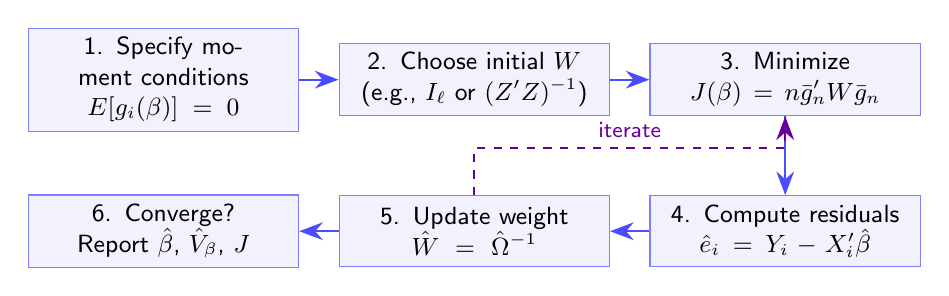
\begin{tikzpicture}[
  node distance=1.0cm and 0.5cm,
  box/.style={rectangle, draw=blue!50, fill=blue!5, text width=3.2cm, minimum height=0.9cm, align=center, font=\small},
  arrow/.style={-{Stealth[length=3mm]}, thick, blue!70}
]

\node[box] (specify) {1. Specify moment conditions\\$\mathbb{E}[g_i(\beta)] = 0$};
\node[box, right=of specify] (choose) {2. Choose initial $W$\\(e.g., $I_\ell$ or $(Z'Z)^{-1}$)};
\node[box, right=of choose] (minimize) {3. Minimize\\$J(\beta) = n\bar{g}_n'W\bar{g}_n$};
\node[box, below=of minimize] (residuals) {4. Compute residuals\\$\hat e_i = Y_i - X_i'\hat\beta$};
\node[box, left=of residuals] (update) {5. Update weight\\$\hat W = \hat\Omega^{-1}$};
\node[box, left=of update] (converge) {6. Converge?\\Report $\hat\beta$, $\hat V_\beta$, $J$};

\draw[arrow] (specify) -- (choose);
\draw[arrow] (choose) -- (minimize);
\draw[arrow] (minimize) -- (residuals);
\draw[arrow] (residuals) -- (update);
\draw[arrow] (update) -- (converge);
\draw[arrow, dashed, darkpurple] (update.north) -- ++(0,0.6) -| (minimize.south) node[pos=0.25, above, font=\footnotesize\color{darkpurple}] {iterate};

\end{tikzpicture}
\end{center}

\smallskip
\begin{itemize}
\item \textbf{One-step:} Stop after step 3 (e.g., 2SLS with $W=(Z'Z)^{-1}$)
\item \textbf{Two-step:} One pass through steps 3--5
\item \textbf{Iterated:} Repeat steps 3--5 until convergence
\end{itemize}

\end{frame}

%--- Slide 28: Key Theorems Summary ---
\begin{frame}{Key Theorems Summary}

\begin{table}[h]
\centering
\small
\begin{tabular}{lp{9cm}}
\toprule
\textbf{Theorem} & \textbf{Result} \\
\midrule
13.1 & GMM estimator (linear): $\hat\beta = (X'ZWZ'X)^{-1}(X'ZWZ'Y)$ \\[3pt]
13.2 & $W = (Z'Z)^{-1}$ gives 2SLS; just-identified gives IV \\[3pt]
13.3 & Asymptotic normality with sandwich variance \\[3pt]
13.4 & Efficient GMM: $W = \Omega^{-1}$, variance $(Q'\Omega^{-1}Q)^{-1}$ \\[3pt]
13.5 & Efficient GMM has smallest variance among GMM estimators \\[3pt]
13.6 & 2SLS is efficient GMM under homoskedasticity \\[3pt]
13.7 & Two-step GMM is asymptotically efficient \\
\bottomrule
\end{tabular}
\end{table}

\medskip
\textbf{Running theme:} These parallel the OLS $\to$ GLS progression. GMM is to IV what GLS is to OLS.

\end{frame}

%--- Slide 29: The Three Meta-Lessons (Part 1) ---
\begin{frame}{The Three Meta-Lessons (Part 1)}

\begin{enumerate}
\item \textbf{Semiparametric}
\begin{itemize}
\item GMM requires only $\mathbb{E}[g_i(\beta)] = 0$ --- no distributional assumptions
\item The missing data application: no assumption on the distribution of missingness, errors, or regressors --- only moment conditions
\item Chamberlain (1987): efficient GMM achieves the semiparametric bound
\end{itemize}

\medskip
\item \textbf{Efficient}
\begin{itemize}
\item Optimal weighting $W = \Omega^{-1}$ minimizes asymptotic variance
\item Missing data: GMM achieves lower MSE than complete case, dummy variable, or imputation
\end{itemize}

\medskip
\item \textbf{General}
\begin{itemize}
\item Nests OLS, IV, 2SLS, GLS as special cases
\item Extends to nonlinear models (missing data, MTE)
\item \textit{Next lecture:} also provides a unified testing framework
\end{itemize}
\end{enumerate}

\end{frame}

%--- Slide 30: Preview of Next Lecture ---
\begin{frame}{Preview of Next Lecture}

\textbf{Lecture 16: GMM Inference and Going Beyond ATE}

\medskip
\begin{itemize}
\item \textbf{Testing:} The J-test for overidentification (Thm 13.14)
\item \textbf{Hypothesis tests:} Wald test and Distance test in the GMM framework
\item \textbf{Subset tests:} Testing specific instruments, endogeneity tests
\item \textbf{Application: Propaganda and Foreign Media}
\begin{itemize}
\item Kern \& Hainmueller: West German TV in East Germany
\item IV gives LATE $\approx -0.12$ (media reduces support for regime)
\item MTE reveals \alert{treatment effect heterogeneity}: always-takers vs.\ never-takers have \textit{opposite signs}
\end{itemize}
\item \textbf{The course in one slide:} OLS $\to$ GLS $\to$ IV $\to$ 2SLS $\to$ GMM
\end{itemize}

\end{frame}

\end{document}
